\documentclass{standalone}
\usepackage{tikz}
\usetikzlibrary{patterns, positioning}

\begin{document}
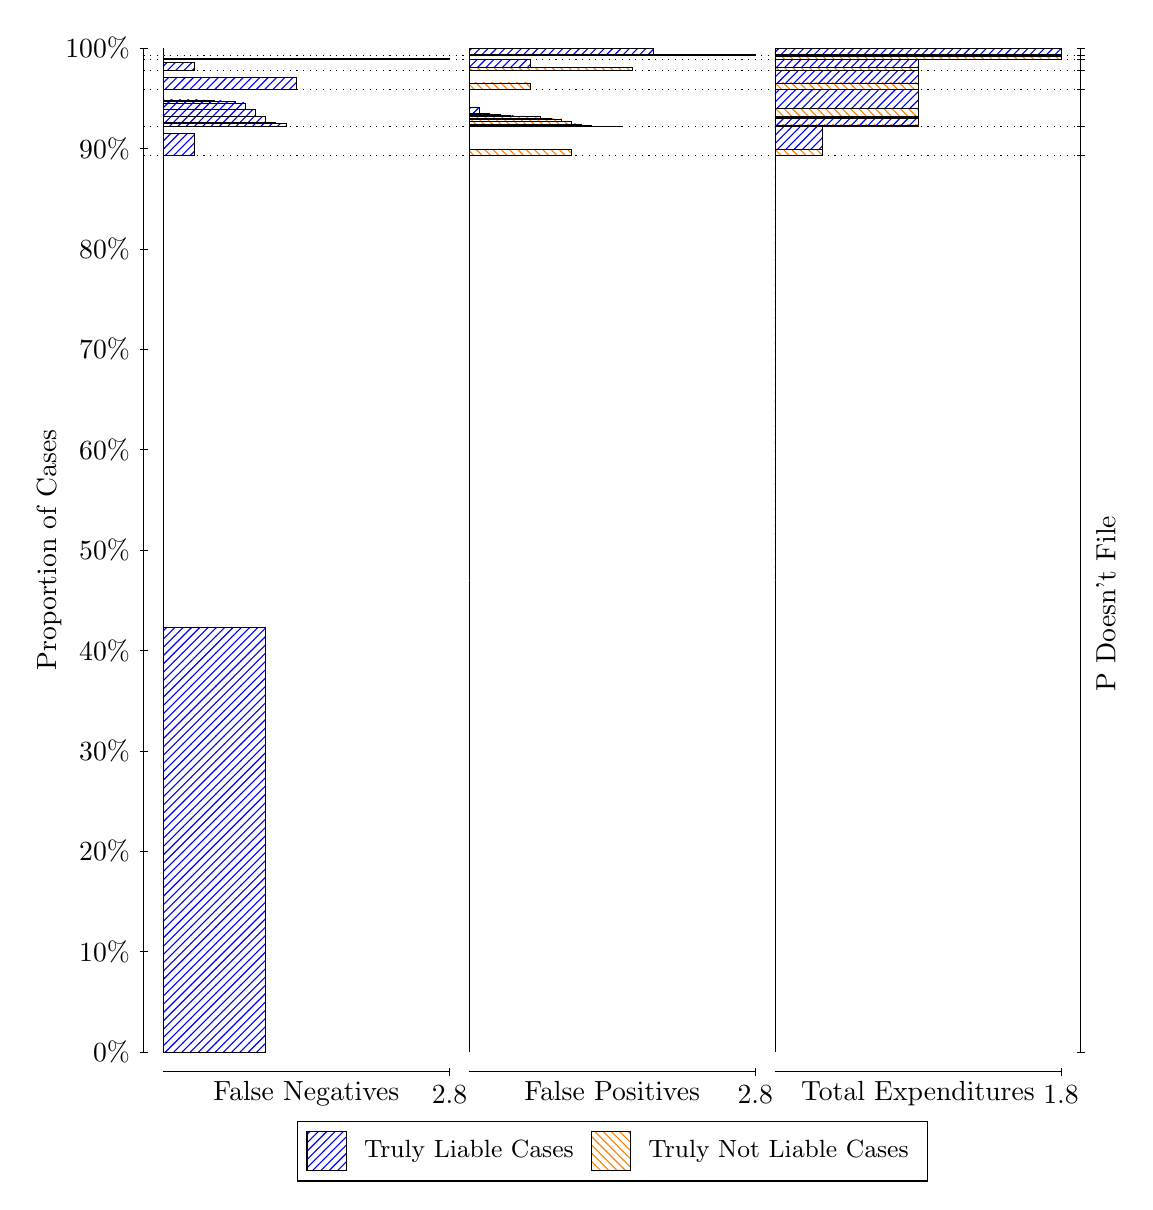
\begin{tikzpicture}
\draw[black, very thin] (1.5,1.75) -- (1.5,14.5);
\node[rotate=90, anchor=center] at (0.3, 8.125) {Proportion of Cases};
\draw[black, very thin] (1.45,1.75) -- (1.55,1.75);
\node[anchor=east] at (1.45, 1.75) {0\%};
\draw[black, very thin] (1.45,3.025) -- (1.55,3.025);
\node[anchor=east] at (1.45, 3.025) {10\%};
\draw[black, very thin] (1.45,4.3) -- (1.55,4.3);
\node[anchor=east] at (1.45, 4.3) {20\%};
\draw[black, very thin] (1.45,5.575) -- (1.55,5.575);
\node[anchor=east] at (1.45, 5.575) {30\%};
\draw[black, very thin] (1.45,6.85) -- (1.55,6.85);
\node[anchor=east] at (1.45, 6.85) {40\%};
\draw[black, very thin] (1.45,8.125) -- (1.55,8.125);
\node[anchor=east] at (1.45, 8.125) {50\%};
\draw[black, very thin] (1.45,9.4) -- (1.55,9.4);
\node[anchor=east] at (1.45, 9.4) {60\%};
\draw[black, very thin] (1.45,10.675) -- (1.55,10.675);
\node[anchor=east] at (1.45, 10.675) {70\%};
\draw[black, very thin] (1.45,11.95) -- (1.55,11.95);
\node[anchor=east] at (1.45, 11.95) {80\%};
\draw[black, very thin] (1.45,13.225) -- (1.55,13.225);
\node[anchor=east] at (1.45, 13.225) {90\%};
\draw[black, very thin] (1.45,14.5) -- (1.55,14.5);
\node[anchor=east] at (1.45, 14.5) {100\%};

\draw[black, very thin] (13.4,1.75) -- (13.4,14.5);
\draw[black, very thin] (13.35,1.75) -- (13.45,1.75);
\node[anchor=west] at (13.35, 1.75) {};
\draw[black, very thin] (13.35,13.133) -- (13.45,13.133);
\node[anchor=west] at (13.35, 13.133) {};
\draw[black, very thin] (13.35,13.501) -- (13.45,13.501);
\node[anchor=west] at (13.35, 13.501) {};
\draw[black, very thin] (13.35,13.973) -- (13.45,13.973);
\node[anchor=west] at (13.35, 13.973) {};
\draw[black, very thin] (13.35,14.216) -- (13.45,14.216);
\node[anchor=west] at (13.35, 14.216) {};
\draw[black, very thin] (13.35,14.354) -- (13.45,14.354);
\node[anchor=west] at (13.35, 14.354) {};
\draw[black, very thin] (13.35,14.405) -- (13.45,14.405);
\node[anchor=west] at (13.35, 14.405) {};
\draw[black, very thin] (13.35,14.5) -- (13.45,14.5);
\node[anchor=west] at (13.35, 14.5) {};

\draw[black, very thin, pattern color=blue, pattern=north east lines] (1.75,1.75) rectangle (3.0476,7.1447);
\draw[black, very thin, pattern color=orange, pattern=north west lines] (1.75,7.1447) rectangle (1.75,13.133);
\draw[black, very thin, pattern color=blue, pattern=north east lines] (1.75,13.133) rectangle (2.1393,13.417);
\draw[black, very thin, pattern color=orange, pattern=north west lines] (1.75,13.417) rectangle (1.75,13.501);
\draw[black, very thin, pattern color=blue, pattern=north east lines] (1.75,13.501) rectangle (3.3071,13.54);
\draw[black, very thin, pattern color=blue, pattern=north east lines] (1.75,13.54) rectangle (3.1774,13.554);
\draw[black, very thin, pattern color=blue, pattern=north east lines] (1.75,13.554) rectangle (3.0476,13.631);
\draw[black, very thin, pattern color=blue, pattern=north east lines] (1.75,13.631) rectangle (2.9179,13.636);
\draw[black, very thin, pattern color=blue, pattern=north east lines] (1.75,13.636) rectangle (2.9179,13.723);
\draw[black, very thin, pattern color=blue, pattern=north east lines] (1.75,13.723) rectangle (2.7881,13.803);
\draw[black, very thin, pattern color=blue, pattern=north east lines] (1.75,13.803) rectangle (2.6583,13.818);
\draw[black, very thin, pattern color=blue, pattern=north east lines] (1.75,13.818) rectangle (2.5286,13.83);
\draw[black, very thin, pattern color=blue, pattern=north east lines] (1.75,13.83) rectangle (2.3988,13.836);
\draw[black, very thin, pattern color=blue, pattern=north east lines] (1.75,13.836) rectangle (2.269,13.841);
\draw[black, very thin, pattern color=orange, pattern=north west lines] (1.75,13.841) rectangle (1.75,13.973);
\draw[black, very thin, pattern color=blue, pattern=north east lines] (1.75,13.973) rectangle (3.4369,14.131);
\draw[black, very thin, pattern color=orange, pattern=north west lines] (1.75,14.131) rectangle (1.75,14.216);
\draw[black, very thin, pattern color=blue, pattern=north east lines] (1.75,14.216) rectangle (2.1393,14.319);
\draw[black, very thin, pattern color=orange, pattern=north west lines] (1.75,14.319) rectangle (1.75,14.354);
\draw[black, very thin, pattern color=blue, pattern=north east lines] (1.75,14.354) rectangle (5.3833,14.37);
\draw[black, very thin, pattern color=orange, pattern=north west lines] (1.75,14.37) rectangle (1.75,14.405);
\draw[black, very thin, pattern color=orange, pattern=north west lines] (1.75,14.405) rectangle (1.75,14.422);
\draw[black, very thin, pattern color=blue, pattern=north east lines] (1.75,14.422) rectangle (1.75,14.5);
\draw[black, very thin, pattern color=orange, pattern=north west lines] (5.6333,1.75) rectangle (5.6333,7.7385);
\draw[black, very thin, pattern color=blue, pattern=north east lines] (5.6333,7.7385) rectangle (5.6333,13.133);
\draw[black, very thin, pattern color=orange, pattern=north west lines] (5.6333,13.133) rectangle (6.931,13.217);
\draw[black, very thin, pattern color=blue, pattern=north east lines] (5.6333,13.217) rectangle (5.6333,13.501);
\draw[black, very thin, pattern color=orange, pattern=north west lines] (5.6333,13.501) rectangle (7.5798,13.503);
\draw[black, very thin, pattern color=orange, pattern=north west lines] (5.6333,13.503) rectangle (7.45,13.505);
\draw[black, very thin, pattern color=orange, pattern=north west lines] (5.6333,13.505) rectangle (7.3202,13.509);
\draw[black, very thin, pattern color=orange, pattern=north west lines] (5.6333,13.509) rectangle (7.1905,13.515);
\draw[black, very thin, pattern color=orange, pattern=north west lines] (5.6333,13.515) rectangle (7.0607,13.538);
\draw[black, very thin, pattern color=orange, pattern=north west lines] (5.6333,13.538) rectangle (6.931,13.567);
\draw[black, very thin, pattern color=orange, pattern=north west lines] (5.6333,13.567) rectangle (6.8012,13.6);
\draw[black, very thin, pattern color=orange, pattern=north west lines] (5.6333,13.6) rectangle (6.6714,13.61);
\draw[black, very thin, pattern color=orange, pattern=north west lines] (5.6333,13.61) rectangle (6.5417,13.632);
\draw[black, very thin, pattern color=blue, pattern=north east lines] (5.6333,13.632) rectangle (6.2821,13.638);
\draw[black, very thin, pattern color=blue, pattern=north east lines] (5.6333,13.638) rectangle (6.1524,13.643);
\draw[black, very thin, pattern color=blue, pattern=north east lines] (5.6333,13.643) rectangle (6.0226,13.655);
\draw[black, very thin, pattern color=blue, pattern=north east lines] (5.6333,13.655) rectangle (5.8929,13.67);
\draw[black, very thin, pattern color=blue, pattern=north east lines] (5.6333,13.67) rectangle (5.7631,13.75);
\draw[black, very thin, pattern color=blue, pattern=north east lines] (5.6333,13.75) rectangle (5.6333,13.973);
\draw[black, very thin, pattern color=orange, pattern=north west lines] (5.6333,13.973) rectangle (6.4119,14.058);
\draw[black, very thin, pattern color=blue, pattern=north east lines] (5.6333,14.058) rectangle (5.6333,14.216);
\draw[black, very thin, pattern color=orange, pattern=north west lines] (5.6333,14.216) rectangle (7.7095,14.251);
\draw[black, very thin, pattern color=blue, pattern=north east lines] (5.6333,14.251) rectangle (6.4119,14.354);
\draw[black, very thin, pattern color=orange, pattern=north west lines] (5.6333,14.354) rectangle (5.6333,14.389);
\draw[black, very thin, pattern color=blue, pattern=north east lines] (5.6333,14.389) rectangle (5.6333,14.405);
\draw[black, very thin, pattern color=orange, pattern=north west lines] (5.6333,14.405) rectangle (9.2667,14.422);
\draw[black, very thin, pattern color=blue, pattern=north east lines] (5.6333,14.422) rectangle (7.969,14.5);
\draw[black, very thin, pattern color=orange, pattern=north west lines] (9.5167,1.75) rectangle (9.5167,7.7385);
\draw[black, very thin, pattern color=blue, pattern=north east lines] (9.5167,7.7385) rectangle (9.5167,13.133);
\draw[black, very thin, pattern color=orange, pattern=north west lines] (9.5167,13.133) rectangle (10.122,13.217);
\draw[black, very thin, pattern color=blue, pattern=north east lines] (9.5167,13.217) rectangle (10.122,13.501);
\draw[black, very thin, pattern color=orange, pattern=north west lines] (9.5167,13.501) rectangle (11.333,13.524);
\draw[black, very thin, pattern color=blue, pattern=north east lines] (9.5167,13.524) rectangle (11.333,13.604);
\draw[black, very thin, pattern color=orange, pattern=north west lines] (9.5167,13.604) rectangle (11.333,13.616);
\draw[black, very thin, pattern color=blue, pattern=north east lines] (9.5167,13.616) rectangle (11.333,13.635);
\draw[black, very thin, pattern color=orange, pattern=north west lines] (9.5167,13.635) rectangle (11.333,13.731);
\draw[black, very thin, pattern color=blue, pattern=north east lines] (9.5167,13.731) rectangle (11.333,13.973);
\draw[black, very thin, pattern color=orange, pattern=north west lines] (9.5167,13.973) rectangle (11.333,14.058);
\draw[black, very thin, pattern color=blue, pattern=north east lines] (9.5167,14.058) rectangle (11.333,14.216);
\draw[black, very thin, pattern color=orange, pattern=north west lines] (9.5167,14.216) rectangle (11.333,14.251);
\draw[black, very thin, pattern color=blue, pattern=north east lines] (9.5167,14.251) rectangle (11.333,14.354);
\draw[black, very thin, pattern color=orange, pattern=north west lines] (9.5167,14.354) rectangle (13.15,14.389);
\draw[black, very thin, pattern color=blue, pattern=north east lines] (9.5167,14.389) rectangle (13.15,14.405);
\draw[black, very thin, pattern color=orange, pattern=north west lines] (9.5167,14.405) rectangle (13.15,14.422);
\draw[black, very thin, pattern color=blue, pattern=north east lines] (9.5167,14.422) rectangle (13.15,14.5);
\draw[black, dotted] (1.5,13.133) -- (13.4,13.133);
\draw[black, dotted] (1.5,13.501) -- (13.4,13.501);
\draw[black, dotted] (1.5,13.973) -- (13.4,13.973);
\draw[black, dotted] (1.5,14.216) -- (13.4,14.216);
\draw[black, dotted] (1.5,14.354) -- (13.4,14.354);
\draw[black, dotted] (1.5,14.405) -- (13.4,14.405);
\draw[black, very thin] (1.75,1.5) -- (5.3833,1.5);
\node[anchor=north] at (3.5667, 1.5) {False Negatives};
\draw[black, very thin] (5.3833,1.45) -- (5.3833,1.55);
\node[anchor=north] at (5.3833, 1.45) {2.8};

\draw[black, very thin] (5.6333,1.5) -- (9.2667,1.5);
\node[anchor=north] at (7.45, 1.5) {False Positives};
\draw[black, very thin] (9.2667,1.45) -- (9.2667,1.55);
\node[anchor=north] at (9.2667, 1.45) {2.8};

\draw[black, very thin] (9.5167,1.5) -- (13.15,1.5);
\node[anchor=north] at (11.333, 1.5) {Total Expenditures};
\draw[black, very thin] (13.15,1.45) -- (13.15,1.55);
\node[anchor=north] at (13.15, 1.45) {1.8};

\node[black, centered, rotate=90] at (13.72, 7.4416) {P Doesn't File};







\draw (7.449999999999999,1.5) node[draw=none] (baseCoordinate) {};
\begin{scope}[align=center]
        \matrix[scale=0.5, draw=black, below=0.5cm of baseCoordinate, nodes={draw}, column sep=0.1cm]{
            \node[rectangle, draw, minimum width=0.5cm, minimum height=0.5cm, pattern=north east lines, pattern color=blue] {}; &
            \node[draw=none, font=\small] (B) {Truly Liable Cases}; &
            \node[rectangle, draw, minimum width=0.5cm, minimum height=0.5cm, pattern=north west lines, pattern color=orange] {}; &
            \node[draw=none, font=\small] (B) {Truly Not Liable Cases}; \\
            };
\end{scope}

\end{tikzpicture}
\end{document}